\documentclass[12pt]{article}
\usepackage[utf8]{inputenc}
\usepackage[T1]{fontenc}
\usepackage[spanish]{babel}
\usepackage{amsmath, amssymb, amsthm}
\usepackage{graphicx}
\usepackage{booktabs}
\usepackage{hyperref}
\usepackage{float}
\usepackage{geometry}
\geometry{a4paper, margin=1in}

\title{Simulación de un Sistema de Colas en Serie \\ (Ejemplo 7.3, \textit{Simulation, Fifth Edition by Sheldon M. Ross})}
\author{Luis Alejandro Arteaga Morales}
\date{\today}

\begin{document}

\maketitle

\section{Introducción}
El objetivo principal de este proyecto es modelar y analizar un sistema de colas en serie en el que cada cliente debe ser atendido por dos servidores dispuestos en tándem (o en serie). La simulación se fundamenta en el enfoque de eventos discretos, donde se consideran eventos tales como la llegada de un cliente y la finalización del servicio en cada servidor.

\subsection{Objetivos}
Este estudio tiene dos objetivos:
\begin{itemize}
    \item Comprender el impacto de las tasas de servicio en el rendimiento global del sistema, medido a través del tiempo promedio que los clientes permanecen en el sistema.
    \item Analizar cómo el sistema se estabiliza en los tiempos promedio al variar el parámetro $\lambda_{max}$ cuando la cantidad de clientes crece.
    \item Evaluar la influencia del balanceo de carga entre los servidores, demostrando que una mayor igualdad entre las tasas de servicio conduce a una menor congestión y tiempos de espera reducidos.
\end{itemize}

\section{Variables, Descripción del Sistema y Detalles de Implementación}
La simulación se implementa siguiendo el esquema propuesto en el Ejemplo 7.3 de \textit{Simulation, Fifth Edition} de Sheldon M. Ross. Se utiliza un modelo de eventos discretos, en el que:
\begin{itemize}
    \item \textbf{Variables clave:}
        \begin{itemize}
            \item \textbf{Tiempo de llegada} (\(t_A\)): definido mediante un proceso de Poisson no homogéneo, que permite capturar variaciones temporales en la intensidad de llegadas. Esto se implementa en el método \texttt{next\_arrival\_time} de la clase \texttt{Simulation}, donde se utiliza una función de intensidad \(\lambda(t)\) para modelar la variabilidad temporal de las llegadas. La función \(\lambda(t)\) está definida como \( \lambda(t) = \lambda_0 \cdot (1 + 0.5 \cdot \sin(2 \pi t / \text{periodo})) \), lo que introduce un patrón cíclico en las llegadas.
            \item \textbf{Tiempos de servicio} en el primer y segundo servidor: denominados \(G_1\) y \(G_2\) respectivamente. En la simulación se emplean distribuciones exponenciales para modelar estos tiempos, utilizando las tasas \(\mu_1\) y \(\mu_2\). Esto se refleja en los cálculos de los tiempos de servicio (\texttt{s1} y \texttt{s2}) mediante la función \texttt{random.expovariate}. La elección de distribuciones exponenciales para \(G_1\) y \(G_2\) se debe a su simplicidad y a su propiedad de falta de memoria, lo que las hace ideales para modelar tiempos de servicio en sistemas de colas.
            \item \textbf{Estados del sistema:} representados por el número de clientes en cada servidor y en cola. En el código, esto se modela mediante las listas \texttt{q1} y \texttt{q2} para las colas, y las variables \texttt{busy1}, \texttt{busy2}, \texttt{cur1}, y \texttt{cur2} para rastrear el estado de los servidores. Estas variables permiten determinar si un servidor está ocupado o libre, así como gestionar la asignación de clientes a los servidores.
        \end{itemize}
        \item \textbf{Eventos:} se consideran tres tipos de eventos: la llegada de un cliente, la finalización del servicio en el primer servidor y la finalización del servicio en el segundo servidor. Cada evento actualiza las variables de estado y registra datos relevantes (tiempos de llegada, inicio y salida). Estos eventos se procesan en un ciclo principal que selecciona el próximo evento a ocurrir en función de los tiempos calculados (\texttt{ta}, \texttt{t1}, \texttt{t2}).
        \item \textbf{Ciclos de simulación:} En el código la cantidad de clientes se controla mediante la variable \texttt{max\_customers}, que define el número total de clientes a procesar antes de finalizar la simulación.
\end{itemize}

La implementación de la simulación se encuentra en el archivo \texttt{simulation.py}. En dicho archivo se define una clase \texttt{Simulation} que encapsula la lógica del modelo. 

\section{Outputs del Sistema}
La simulación implementada en el archivo \texttt{simulation.py} genera como salida principal un diccionario que contiene información detallada sobre cada cliente procesado en el sistema. Este diccionario incluye los siguientes datos para cada cliente:

\begin{itemize}
    \item \textbf{Tiempo de llegada al sistema:} el instante en que el cliente llega al primer servidor.
    \item \textbf{Inicio del servicio en el primer servidor:} el momento en que el cliente comienza a ser atendido en el primer servidor.
    \item \textbf{Finalización del servicio en el primer servidor:} el instante en que el cliente termina de ser atendido en el primer servidor.
    \item \textbf{Tiempo de llegada al segundo servidor:} el momento en que el cliente llega al segundo servidor tras finalizar su servicio en el primero.
    \item \textbf{Inicio del servicio en el segundo servidor:} el instante en que el cliente comienza a ser atendido en el segundo servidor.
    \item \textbf{Finalización del servicio en el segundo servidor:} el momento en que el cliente termina de ser atendido en el segundo servidor y abandona el sistema.
\end{itemize}

Además, se calculan métricas agregadas a partir de estos datos, tales como:
\begin{itemize}
    \item \textbf{Tiempo total en el sistema:} el tiempo transcurrido desde la llegada del cliente al sistema hasta su salida final.
    \item \textbf{Tiempo total en el primer servidor:} el tiempo que el cliente pasa en el primer servidor, incluyendo el tiempo de espera en la cola.
    \item \textbf{Tiempo total en el segundo servidor:} el tiempo que el cliente pasa en el segundo servidor, incluyendo el tiempo de espera en la cola.
\end{itemize}

Con estos resultados se puede evaluar el impacto de los distintos parámetros de la simulación en las métricas clave.

\section{Resultados y Experimentos}
\subsection{Impacto de \texorpdfstring{$\lambda_{max}$}{lambda\_max} y \texorpdfstring{\textit{max\_customers}}{max\_customers}. Estabilización del Sistema}

El primer análisis se centró en estudiar el impacto del parámetro $\lambda_{max}$ (tasa máxima de llegadas) en el tiempo promedio que los clientes pasan en el sistema, considerando diferentes valores de \texttt{max\_customers}.

\subsubsection{Resultados Observados e Interpretación}
Se observó que, para valores pequeños de \texttt{max\_customers}, el tiempo promedio en el sistema es más sensible a las variaciones de $\lambda_{max}$. Esto se debe a que, con un número reducido de clientes, las fluctuaciones en las llegadas y los tiempos de servicio tienen un impacto más pronunciado en las métricas agregadas. Sin embargo, a medida que \texttt{max\_customers} aumenta, el sistema tiende a estabilizarse, y el tiempo promedio en el sistema converge hacia un valor constante, independientemente de las variaciones en $\lambda_{max}$. Este valor parece estar cerca de 7.6s.

\begin{figure}[H]
    \centering
    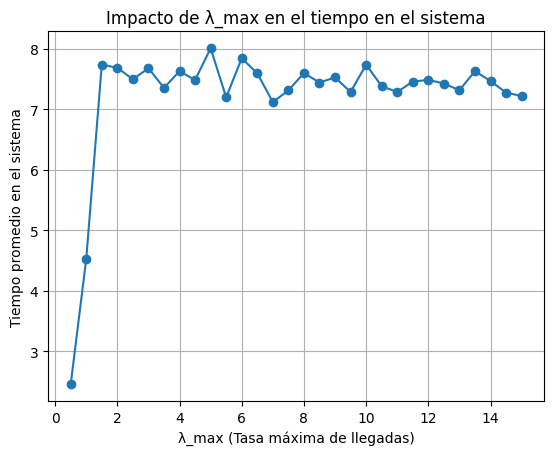
\includegraphics[width=0.8\textwidth]{results1.0.png}
    \caption{Comparación de tiempos promedio en el sistema para diferentes configuraciones de \texttt{max\_customers}. y \texttt{lambda\_max=1.5}.}
    \label{fig:results1.0}
\end{figure}

\begin{figure}[H]
    \centering
    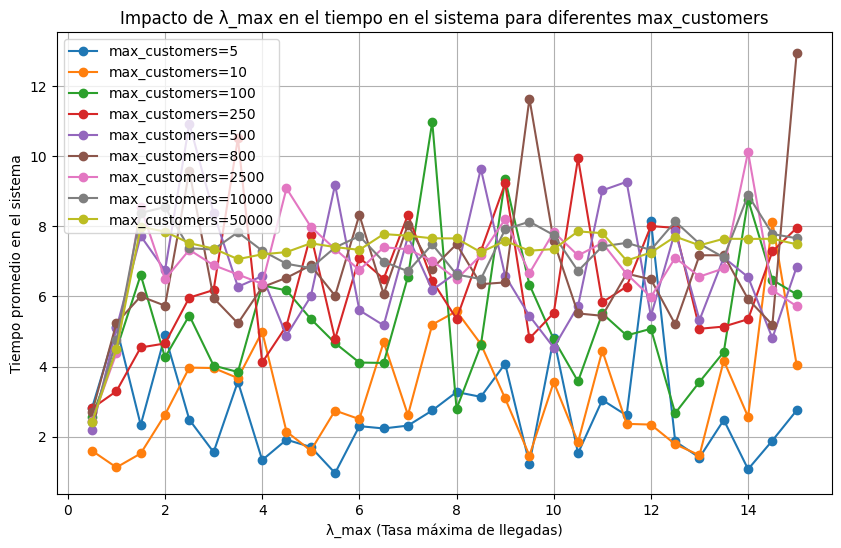
\includegraphics[width=0.8\textwidth]{results1.1.png}
    \caption{Comparación de tiempos promedio en el sistema para diferentes configuraciones de \texttt{max\_customers} y \texttt{lambda\_max}.}
    \label{fig:results1.1}
\end{figure}

\subsubsection{Implicaciones Prácticas}
Estos resultados tienen implicaciones importantes para el diseño y la gestión de sistemas de colas en serie. En particular:
\begin{itemize}
    \item Para sistemas con un volumen alto de clientes, las métricas de rendimiento pueden predecirse con mayor precisión, lo que facilita la planificación y optimización.
    \item En sistemas con un número reducido de clientes, es crucial considerar la sensibilidad a las variaciones en las tasas de llegada, ya que estas pueden tener un impacto significativo en el rendimiento.
\end{itemize}

\subsection{Variación de las tasas de servicio \texorpdfstring{$\mu_1$}{mu1} y \texorpdfstring{$\mu_2$}{mu2}}
Para evaluar el impacto de las tasas de servicio (\(\mu_1\) y \(\mu_2\)) sobre el rendimiento del sistema, se realizaron experimentos de análisis de sensibilidad utilizando un notebook de Jupyter (\texttt{results.ipynb}). En estos experimentos se varían las tasas de servicio y se observan los siguientes indicadores:
\begin{itemize}
    \item \textbf{Tiempo total en el sistema:} se mide el tiempo transcurrido desde la llegada del cliente hasta su salida final tras ser atendido por ambos servidores.
    \item \textbf{Longitud de las colas y balanceo de carga:} se evalúa de forma indirecta mediante el tiempo promedio de servicio en cada servidor.
\end{itemize}

Entre los experimentos realizados se destacan los siguientes casos:
\begin{itemize}
    \item \textbf{Caso balanceado:} \(\mu_1 = \mu_2\) (por ejemplo, 1.0, 1.5, 2.0 y 2.5). Estos casos demuestran que, cuando ambos servidores tienen capacidades similares, se minimiza el tiempo total que los clientes pasan en el sistema.
    \item \textbf{Casos desbalanceados:} \(\mu_1 \neq \mu_2\), donde un servidor es significativamente más rápido que el otro. Estos escenarios muestran que el desequilibrio en las tasas de servicio incrementa la congestión, ya que se genera una acumulación de clientes en el servidor con menor tasa.
\end{itemize}

Los resultados se resumen en un gráfico de barras, que evidencia que las configuraciones balanceadas (donde \(\mu_1 \approx \mu_2\)) presentan tiempos promedio en el sistema considerablemente menores, lo que respalda la hipótesis de que la igualdad en las capacidades de los servidores optimiza el rendimiento global.

\begin{figure}[H]
    \centering
    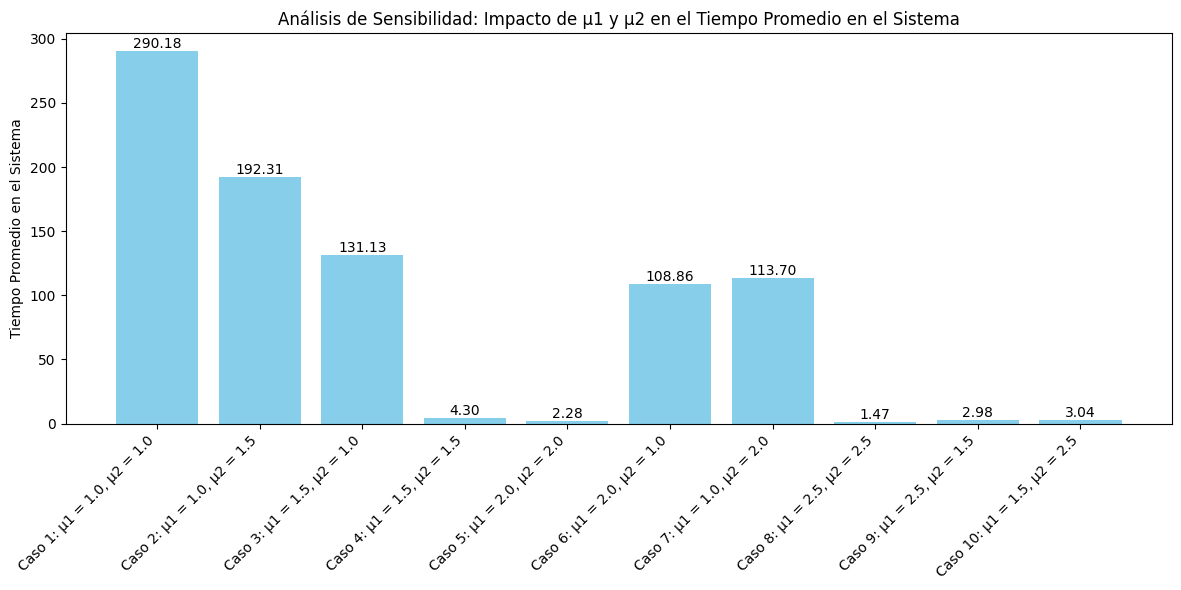
\includegraphics[width=0.9\textwidth]{results2.png}
    \caption{Resultados del análisis de sensibilidad: tiempo promedio en el sistema en función de las tasas de servicio \(\mu_1\) y \(\mu_2\).}
    \label{fig:results2}
\end{figure}

\section{Modelo Matemático y Supuestos}
El modelo se fundamenta en:
\begin{itemize}
    \item Un proceso de llegadas no homogéneo, definido mediante una función de intensidad \( \lambda(t) \), que captura la variabilidad temporal de las llegadas.
    \item Distribuciones de servicio \( G_1 \) y \( G_2 \) para cada servidor. Aunque en la implementación se utilizaron distribuciones exponenciales, el modelo es general y permite otras formas de distribución, siempre y cuando se mantenga la independencia de las llegadas y de los tiempos de servicio.
    \item La política de atención \textit{primero en llegar, primero en ser atendido} (FCFS) en cada cola.
\end{itemize}

\section{Conclusiones}
El análisis realizado confirma que:
\begin{itemize}
    \item La variación en las tasas de servicio (\(\mu_1\) y \(\mu_2\)) tiene un impacto significativo en el rendimiento del sistema. En particular, configuraciones balanceadas (con valores similares para ambos parámetros) reducen la congestión y optimizan el tiempo total en el sistema.
    \item El sistema tiende a estabilizarse a medida que aumenta el número de clientes, lo que sugiere que, en escenarios de alta carga, las métricas de rendimiento se vuelven más predecibles y menos sensibles a las variaciones en las tasas de llegada.
\end{itemize}

\section*{Referencias}
\begin{itemize}
    \item Ross, S. M. (2013). \textit{Simulation, Fifth Edition: Statistical Modeling and Decision Science}. Elsevier.
\end{itemize}

\end{document}
